\section {Selecting reaction to perform}
\label{sec:reaction_selection}

We start with the second step of the SSA, selecting a reaction given some propensities. Most algorithms presented here are reviewed in~\citet{gillespie_perspective:_2013}.

Formally, the problem is quite simple: we are given a set of $N$ real values $\{ r_1, r_2, ..., r_N \}$ and we draw index $i$ with probability $p_i = r_i / \sum r_i$. Mathematically, this is a multinomial distribution and thus could be drawn as such by any standard random number library.

We will start by stating a standard technique to perform mulitnomial drawings. We will then introduce methods that increase the speed of the drawing by using \textit {a priori} knowledge.

\subsection {Direct method}

\subsubsection {Principle}

The first method that was used historically is staightforward and sometimes referred to as \textit {biased wheel}. Schematically speaking, you could imagine a wheel similar to ``wheel of fortune'', except the size allowed to each index on the wheel is proportional to its propensity value, so that large value have a larger probability to be drawn when the wheel is spinned~\reffigp{fig:biased_wheel}.

\begin{figure}[!h]
  \centering
  \begin{minipage}{\textwidth}
    \begin{minipage}{0.5\textwidth}
      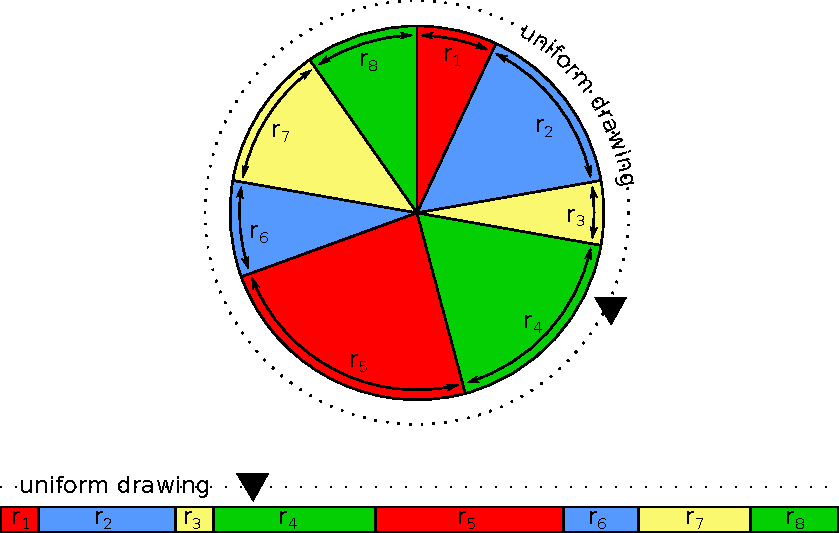
\includegraphics[width=\textwidth]{biased_wheel}
    \end{minipage}
    \begin{minipage}{0.5\textwidth}
      \includegraphics[width=\textwidth]{ratevector_container}
      \includegraphics[width=\textwidth]{ratevector_drawing}
      \includegraphics[width=\textwidth]{ratevector_update}
    \end{minipage}
  \end{minipage}
  \caption{(Left) Illustration of drawing along a biased wheel and its equivalent representation as a segment. (Right) Container and algorithms used to maintain the structure.}
  \label{fig:biased_wheel}
\end {figure}

Generally the wheel is seen as a segment subdivided into $N$ subsegments of length $r_1$, ..., $r_N$. A value $u$ is drawn on this $[0, \sum r_i)$ segment. We proceed iteratively to find to which subsegment $u$ belongs. If $u < r_1$, it belongs to subsegment 1. If $r_1 \leq u < r_1+r_2$, it belongs to subsegment 2, etc.

\subsubsection {Sketch of algorithm and complexity} 

\begin{figure}[!h]
  \begin{minipage}{0.5\textwidth}
    \includegraphics[width=\textwidth]{ratevector_drawing}
  \end{minipage}
  \begin{minipage}{0.5\textwidth}
    \begin{algorithm}[H]
      \KwData{Array r of size N, R = sum (r).}
      \KwResult{Index drawn according to multinomial drawing.}
      u = uniform ([0, R))\;
        index = 1\;
        cum\_sum = r[1]\;
        \While{u $\geq$ cum\_sum}{
          index = index + 1\;
          cum\_sum = cum\_sum + r [index]\;
        }
        \KwRet{index}
    \end{algorithm}
  \end{minipage}
  \caption{Direct drawing method}
  \label{fig:direct_drawing}
\end {figure}

Worst case of the drawing~\reffigp{fig:direct_drawing} occurs when $u$ is in the last subsegment, so the loop has to be iterated $N$ times, yielding $O(N)$ complexity.

\subsection {Next reaction method}

The next reaction method is based on the direct method. It is used in systems where it is known that propensities are not uniform. The point is to accelerate the direct method by sorting (at least rougly) propensities within the vector. This does not change drawing statistics but accelerates finding where a drawing is located on the wheel. For example, say a propensity takes up 50\% of total propensity and is located at the beginning of the vector. Then each random drawing $u < 0.5\sum r_i$ will be instantly found to fall into the first sector of the biased wheel. In a non-sorted vector, we would have to loop through several small sectors before finding the big one.

Because the next reaction method is only a twist of the direct method, we do not go into furter details now. We will also omit it in complexity analysis, as it has the same worst-case complexity as the direct method. We will only reference it again in the Experiment section.

\subsection {Binary tree}

\subsubsection {Principle}

In this approach, we organize propensities inside a tree. Propensities are placed in the leaves of the tree. Nodes are then assembled iteratively 2 by 2 to compute the sum of all propensities~\reffigp {fig:binary_tree}.

\begin{figure}[!h]
  \centering
  \begin{minipage}{0.8\textwidth}
    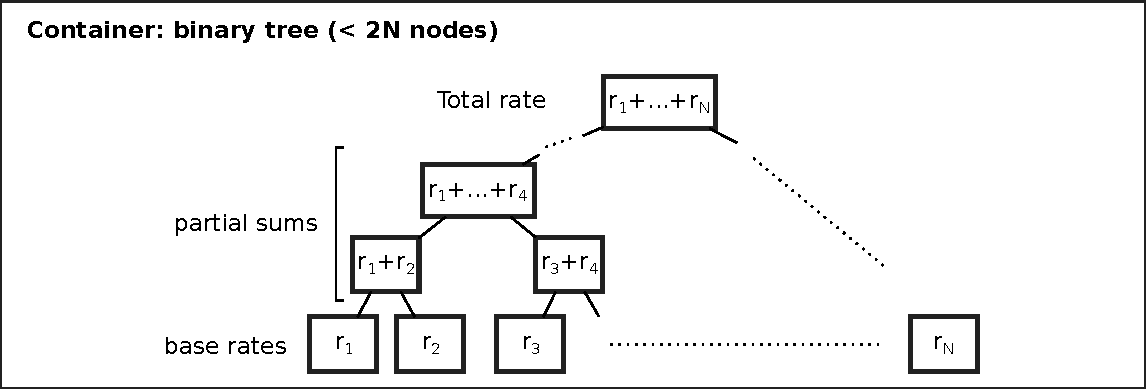
\includegraphics[width=\textwidth]{ratetree_container}
    \includegraphics[width=0.5\textwidth]{ratetree_drawing}
    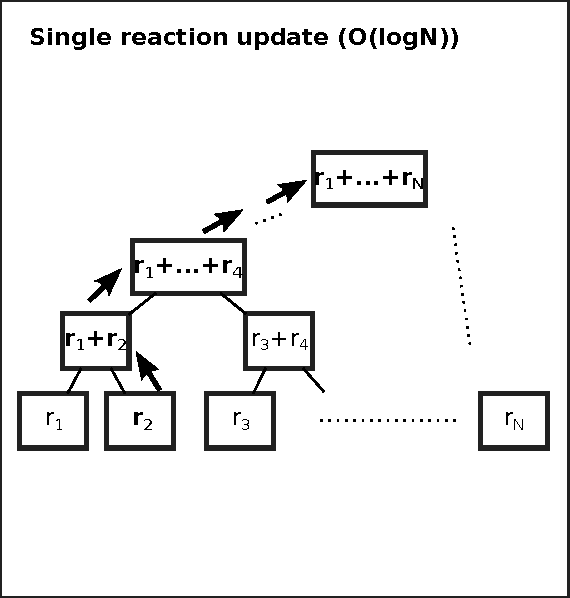
\includegraphics[width=0.5\textwidth]{ratetree_update}
  \end{minipage}
  \caption {Binary tree containing propensities. Propensity values are found at the leaves of the tree. Intermediate nodes represent partial sums of nodes below, root holds the sum of all propensities.}
  \label {fig:binary_tree}
\end {figure}

The idea is that with the structure \emph{in place}, finding the index that has been drawn is quicker. Similarly to the standard drawing, a value $u$ is drawn on the $[0, R=\sum r_i)$ segment. We start from the root node and need to find on which side of the tree $u$ lies. The two children nodes summarize how much weight there is on each side of the tree, say $w_\textrm{left}$ and $w_\textrm{right}$ respectively. If $u < w_\textrm{left}$, we descend to the left child node and proceed the same way until we reach a leaf. If $u \geq w_\textrm{left}$, we descend to the right child and we proceed iteratively with $u = u - w_\textrm{left}$.

This procedure is actually very similar to the biased wheel method, except we perform some kind of progressive zooming in on the subsegments delimited by the propensity values~\reffigp {fig:binary_tree}.

\subsubsection {Sketch of algorithm and complexity} 
\begin{figure}[!h]
  \begin{minipage}{0.5\textwidth}
    \includegraphics[width=\textwidth]{ratetree_drawing}
  \end{minipage}
  \begin{minipage}{0.5\textwidth}
    \begin{algorithm}[H]
      \SetAlgoLined
      \KwData{Binary tree with propensities at its leaves.}
      \KwResult{Index drawn according to multinomial drawing.}
      u = uniform ([0, tree.root.value))\;
        node = tree.root\;
        \While{node is not a leaf}
              {
                \eIf {u $<$ node.left\_child.value}{
                  node = node.left\_child\;
                }{
                  node = node.right\_child\;
                  u = u - node.left\_child.value\;
                }
              }
              \KwRet{node.index}
    \end{algorithm}
  \end{minipage}
  \caption{Binary tree: drawing method.}
  \label{fig:tree_drawing}
\end{figure}

Complexity for performing the drawing~\reffigp{fig:tree_drawing} is given by the depth of the tree, $\lceil\log_2 N\rceil$, which is $O(\log N)$.

\begin{figure}[!h]
  \begin{minipage}{0.5\textwidth}
    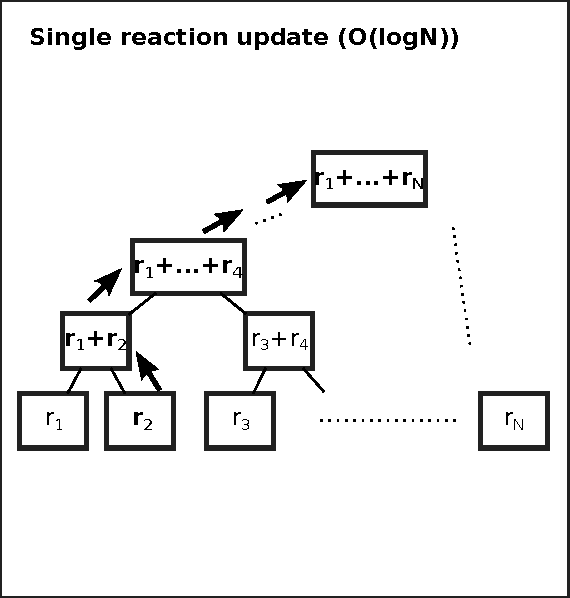
\includegraphics[width=\textwidth]{ratetree_update}
  \end{minipage}
  \begin{minipage}{0.5\textwidth}
    \begin{algorithm}[H]
      \SetAlgoLined
      \KwData{Binary tree with propensities at its leaves. Index i\_update of propensity to update, new propensity value p\_update.}
      \KwResult{Updated binary tree.}
      node = tree.leaf [i\_update]\;
      node.value = p\_update\;
      \While{node is not root}
            {
              node = node.parent\;
              node.value = node.left\_child.value + node.right\_child.value\;
            }
    \end{algorithm}
  \end{minipage}
  \caption{Binary tree: update method.}
  \label{fig:tree_update}
\end{figure}

Complexity for updating the tree~\reffigp{fig:tree_update} is also given by depth of the tree, $O(\log N)$. Note that we need not update every node in the tree, only the parents of the updated leaf up to the root node.


\subsection {Hybrid method}

\subsubsection {Principle}

In this approach, we organize propensities into groups and use a different drawing method: \emph{rejection-base drawing}. This approach has been presented in~\citet{slepoy_constant-time_2008}.

\paragraph{Rejection-based drawing} The aim is to perform a multinomial drawing, similar to what is done by a biased wheel or a binary tree. The problem with the latter methods is that we need to iterate through some structure before finding the right value. With rejection-based drawing, we attempt to \emph{jump} to the right solution. Let $\{r_i\}$ be the propensities of the $N$ reactions in the system and $R = \sum_{1 \leq i \leq N} r_i$.
\begin{enumerate}
\item We choose a value $r_M$ such that $\forall i, r_M \geq r_i$.
\item Until a good candidate is found.
  \begin{enumerate}
  \item We draw a random number $i$ between 1 and $N$ (with replacement).
  \item We draw a random number $u$ on the $[0, r_M]$ segment. If $u > r_i$, we reject $i$, else we keep it.
  \end{enumerate}
\end{enumerate}

A careful proof shows that the probability of drawing index $i$ is equal to $r_i / R$~\citep{serebrinsky_physical_2011}. Note that the choice of $r_M$ is critical for the efficiency of the method~\reffigp[A]{fig:rejection_based_drawing}. Formally, the probability to accept a candidate is $\sum_i\prob{\textrm{draw }i}$ $\prob{\textrm{accept }i} = \sum_i1/N \times r_i/r_M = R/(Nr_M)$. If applied naively, the number of candidates to loop through is a geometric law with parameter $R/(Nr_M)$. The expected number of candidates is thus $Nr_M/R$. For a uniform distribution, this value can be 1, but in general, it yields bad results~\reffigp[B]{fig:rejection_based_drawing}.

\begin{figure}[!h]
  \centering
  \begin{minipage}{0.59\textwidth}
    \textbf{A} \\
    \includegraphics[width=\textwidth]{rejection_principle}
  \end{minipage}
  \begin{minipage}{0.39\textwidth}
    \textbf{B} \\
    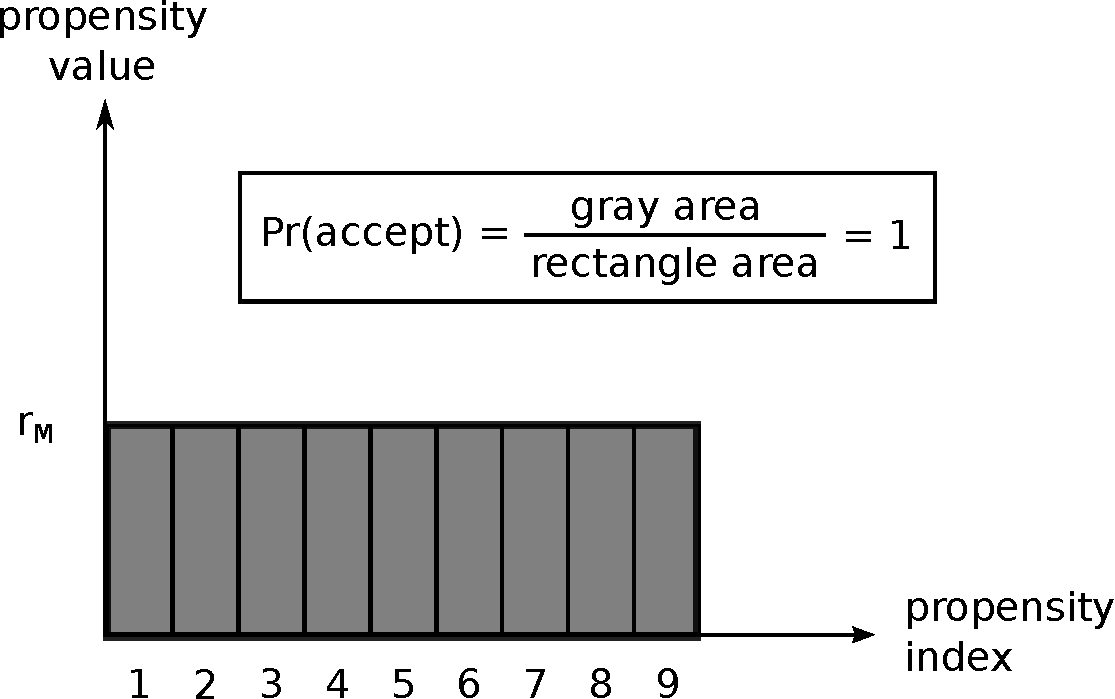
\includegraphics[width=\textwidth]{rejection_uniform}
    \includegraphics[width=\textwidth]{rejection_bad}
  \end{minipage}
  \begin{minipage}{0.6\textwidth}
    \textbf{C}\\
    \includegraphics[width=\textwidth]{rejection_groups}  
  \end{minipage}
  \caption{Rejection based drawing (adapted from \citet{slepoy_constant-time_2008}). (A) Geometric illustration of rejection principle. Drawing occurs in a 2D space, with propensities aligned along the $x$ axis and their value given by gray bars along the $y$ axis. A drawing is accepted if it falls into the gray domain. Note that the probability to draw a propensity is proportional to its value, as an accepted drawing will be distributed uniformly across the gray domain. (B) Examples displaying efficiency of the technique (maximal for uniform propensities, minimal when some are very high and most are very low). (C) Sorting propensities into groups whose limits are powers of 2 ensures a minimal 1/2 acceptation probability \emph{within a given group}.}
  \label{fig:rejection_based_drawing}
\end {figure}

 \paragraph{Group method} The idea behind the algorithm is to improve the acceptation probability by placing propensities in \emph{groups}:
\begin{enumerate}
\item We draw a group index by using a classical method (biased wheel or binary tree).
\item We draw a propensity inside the group by using the rejection-based method.
\end{enumerate}

\citet{slepoy_constant-time_2008} propose placing propensities into binary groups. They choose a base rate $b$. Groups are of the form $(0, b]$, $(b, 2b]$, $(2b, 4b]$, \textit{etc.} $(0,b]$ contains all propensities between 0 and $b$, and so on. When applying the rejection method to any of these groups (except $(0, b]$), the acceptation probability is $\geq 1/2$~\reffigp[C]{fig:rejection_based_drawing}. Note that the number of groups $K$ does not generally depend on $N$, it only depends on the highest propensity value. In general, it remains relatively small.

Suppose the structure is already in place, \textit{i.e.} propensities are placed in the right group and the total propensity for each group is known. Step 1 is at most $O(K)$, which is independent of $N$. Step 2 requires less than 2 candidates on average, so it is $O(1)$. This results in $O(1)$ globally, making it significantly more efficient than the two previous methods. However, we will see that its implementation is also trickier in order to preserve this theoretical complexity.

\begin{figure}[!h]
  \centering
  \includegraphics[width=0.8\textwidth]{hybrid_container}
  \includegraphics[width=0.8\textwidth]{hybrid_drawing}
  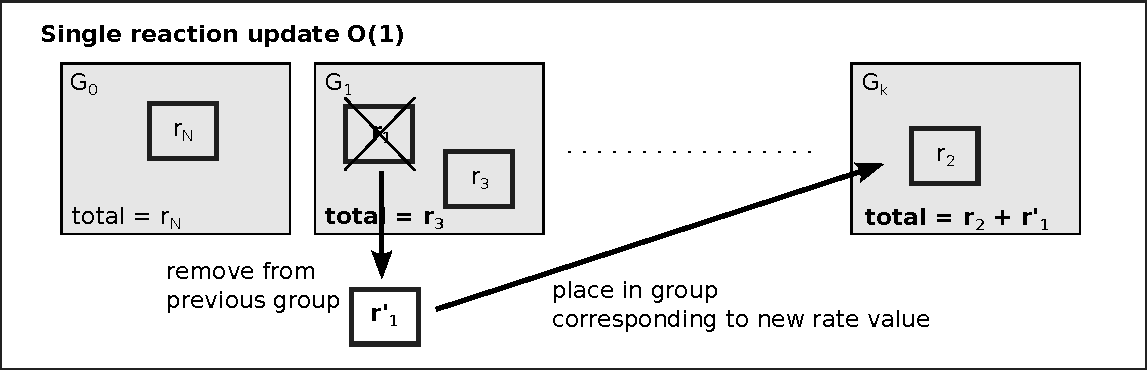
\includegraphics[width=0.8\textwidth]{hybrid_update}
  \caption {Hybrid method using group structure and rejection algorithm.}
  \label {fig:hybrid_method}
\end {figure}

\subsubsection {Sketch of algorithm and complexity} 

\begin{figure}[!h]
  \centering
  \begin{minipage}{\textwidth}
    \centering
    \includegraphics[width=0.8\textwidth]{hybrid_drawing}
    \begin{algorithm}[H]
      \SetAlgoLined
      \KwData{$K+1$ groups, group k containing propensities whose value falls in the interval $(0,b]$ if k=0, $(2^{k-1}b, 2^kb]$ if k $>$ 0. Propensities are stored as a couple containing their value and original index.}
      \KwResult{Index drawn according to multinomial drawing.}
      \tcp {drawing using a direct method like binary tree or biased wheel}
      group = groups [multinomial (group[0].total\_propensity, ..., 
        group[K].total\_propensity)]\;
      \Repeat{candidate.value $>$ uniform (0, group.max\_propensity)}{
        candidate = group.propensities [uniform (1, group.number\_propensities)]\;
      }
      \KwRet{candidate.index}
    \end{algorithm}
  \end{minipage}
  \caption{Hybrid method: drawing method.}
  \label{fig:hybrid_drawing}
\end{figure}

Because of the group structure, the loop in \reffigt{fig:hybrid_drawing} is $O(1)$ (see above). The first multinomial drawing is at most $O(K)$, so the complexity is globally $O(K)$. Because $K$, the number of groups, does not naturally scale with $N$, the number of reactions, the complexity is overall $O(1)$, as $N$ is the real variable of interest here.


\begin{figure}[!h]
  \centering
  \begin{minipage}{\textwidth}
    \centering
    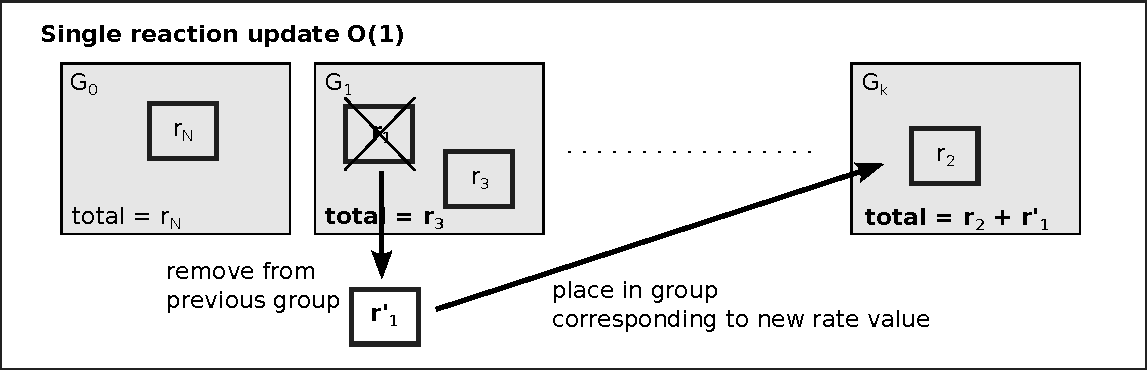
\includegraphics[width=0.8\textwidth]{hybrid_update}
    \begin{algorithm}[H]
      \SetAlgoLined
      \KwData{$K+1$ groups, group k containing propensities whose value falls in the interval $(0,b]$ if k=0, $(2^{k-1}b, 2^kb]$ if k $>$ 0. Propensities are stored as a couple containing their value and original index. Index i\_update of propensity to update, new propensity value p\_update.}
  \KwResult{Updated group structure.}
  \Fn {group\_index (propensity)}{
    \eIf{propensity $\geq$ b}{
      \KwRet{$\lceil \log_2 (\textrm{reaction.propensity} / b) \rceil$}
    }{
      \KwRet {0}
    }
  }
  propensity = propensity corresponding to index i\_update\;
  previous\_group = groups [group\_index (propensity.value)]\;
  Remove propensity from previous\_group and update group's total propensity\;
  new\_group = groups [group\_index (p\_update)]\;
  propensity.value = p\_update\;
  Add propensity to new\_group and update group's total propensity\;
    \end{algorithm}
  \end{minipage}
  \caption{Hybrid method: update method.}
  \label{fig:hybrid_update}
\end{figure}

At first sight, updating the group structure is also $O(1)$~\reffigp{fig:hybrid_update}. However, the parts about removing or inserting a reaction into a group must be carefully implemented in order to achieve that result.

\subsection {Summary}

\reftabt{tab:selection_summary} summarizes the worst case complexity of four methods presented. Note that the update complexity was derived in the case where onle one propensity needed to be updated. To obtain the overall complexity, we need to take into account the number of reactions $U$ whose propensity needs to be updated. A naive analysis indicates that the binary tree could be less efficient than the direct method depending on $U$ and $N$~\reftabp{tab:selection_summary}. In the next section, we will analyze how $U$ can influence the efficiency of each method.

\begin{table}[!h]
  \centering
  \begin{tabular}{|l|c|c|c|}
    \hline
    Method & Drawing Complexity & Update Complexity & Total Complexity\\
           &                    & (one propensity) & \\
    \hline
    Direct Method & $O(N)$ & $O(1)$ & $O(N)$?\\
    Binary Tree & $O(\log N)$ & $O(\log N)$ & $O(U\log N)$?\\
    Hybrid Method & $O(1)$ & $O(1)$ & $O(U)$?\\
    \hline
  \end{tabular}
  \caption{Comparison of worst-case complexities of methods presented here. $N$ is the number of reactions in the system, $U \leq N$ the number of reactions whose propensity needs to be updated. The last column is a projection based on the first two columns, real total complexities are given in the next section.}
  \label{tab:selection_summary}
\end{table}	
